\section{Tổ chức thành phần hệ thống}
\label{sec:system-component-organization}
\begingroup
\sloppy

ProLearning Platform được tổ chức theo hướng phân lớp kết hợp phân rã theo miền nghiệp vụ. Ở mức tổng quan, client chỉ đảm nhiệm giao diện và trạng thái hiển thị; Spring Boot API là nơi tập trung xử lý nghiệp vụ, xác thực, phân quyền và điều phối tích hợp; các dịch vụ hạ tầng được đặt phía sau service/adapter riêng để giảm phụ thuộc trực tiếp giữa domain logic và API bên ngoài~\cite{springbootdocs,springsecurityjwt}.

Sau đây là bảng~\ref{tab:core-component-organization} và Bảng~\ref{tab:support-component-organization} tóm tắt các nhóm thành phần chính trong hệ thống.

\begin{table}[htbp]
    \centering
    \small
    \caption{Tổ chức các thành phần nghiệp vụ chính}
    \label{tab:core-component-organization}
    \renewcommand{\arraystretch}{1.15}
    \begin{tabular}{|p{0.24\textwidth}|p{0.20\textwidth}|p{0.44\textwidth}|}
        \hline
        \textbf{Nhóm thành phần} & \textbf{Vai trò} & \textbf{Chức năng tiêu biểu} \\
        \hline
        Client layer & Giao diện tương tác và gọi API backend. & Web phục vụ quản lý học liệu; mobile phục vụ phiên học ngắn, nhắc học và push notification. REST API là kênh chính; WebSocket/STOMP dùng cho realtime~\cite{springwebsocketstomp}. \\
        \hline
        Security and identity & Xác thực và kiểm soát quyền truy cập. & Đăng ký, đăng nhập, JWT, Google OAuth, role-based access và kiểm tra quyền trên tài nguyên học tập~\cite{springsecurityjwt}. \\
        \hline
        Learning workspace & Quản lý không gian học tập. & Set, folder, note, flashcard, exam, roadmap, file đính kèm, chia sẻ tài nguyên và quyền cộng tác. \\
        \hline
        AI learning & Sinh nội dung và cá nhân hóa học tập. & Tạo flashcard, đề kiểm tra, giải thích ghi chú, phân tích kết quả và tạo roadmap thông qua AI Service nội bộ. \\
        \hline
        Collaboration & Hỗ trợ học tập/cộng tác chung. & Chia sẻ note/set, kiểm tra quyền truy cập và đồng bộ chỉnh sửa ghi chú theo thời gian thực. \\
        \hline
        Review and progress & Theo dõi quá trình học. & Lưu attempt, review log, mastery, lịch ôn flashcard và thống kê tiến độ theo topic. \\
        \hline
    \end{tabular}
\end{table}

\begin{table}[htbp]
    \centering
    \small
    \caption{Tổ chức các thành phần hỗ trợ và hạ tầng}
    \label{tab:support-component-organization}
    \renewcommand{\arraystretch}{1.15}
    \begin{tabular}{|p{0.24\textwidth}|p{0.20\textwidth}|p{0.44\textwidth}|}
        \hline
        \textbf{Nhóm thành phần} & \textbf{Vai trò} & \textbf{Chức năng tiêu biểu} \\
        \hline
        Planning and notification & Quản lý kế hoạch và nhắc học. & Todo, goal, pomodoro, reminder, weekly summary, notification trong ứng dụng, email và push notification. \\
        \hline
        Payment and subscription & Quản lý nâng cấp tài khoản. & Tạo payment link, nhận webhook, xác minh giao dịch, lưu transaction và cập nhật subscription qua PayOS~\cite{payoswebhook}. \\
        \hline
        Admin and moderation & Hỗ trợ vận hành nền tảng. & Quản lý tài khoản, khóa/mở khóa người dùng, onboarding analytics và xử lý appeal. \\
        \hline
        Application boundary & Chuẩn hóa request/response. & Controller, DTO, mapper, validation, exception handler và response wrapper. \\
        \hline
        Support services & Cơ chế dùng chung trong backend. & Permission service, logging, error handling, scheduler, cache helper và xử lý bất đồng bộ. \\
        \hline
        Infrastructure and integration & Lưu trữ và kết nối dịch vụ ngoài. & PostgreSQL, Redis, RabbitMQ, Cloudinary, Firebase Cloud Messaging, Google Calendar, PayOS và SMTP provider. \\
        \hline
    \end{tabular}
\end{table}

Hình~\ref{fig:prolearning-architecture-detail-components} minh họa cách các nhóm thành phần trên liên kết với nhau trong kiến trúc chi tiết. Các dependency nghiệp vụ được định hướng đi qua application layer, trong khi kết nối với dịch vụ ngoài được đóng gói bằng adapter/service chuyên biệt để dễ thay thế, kiểm thử và kiểm soát lỗi.

\begin{figure}[htbp]
    \centering
    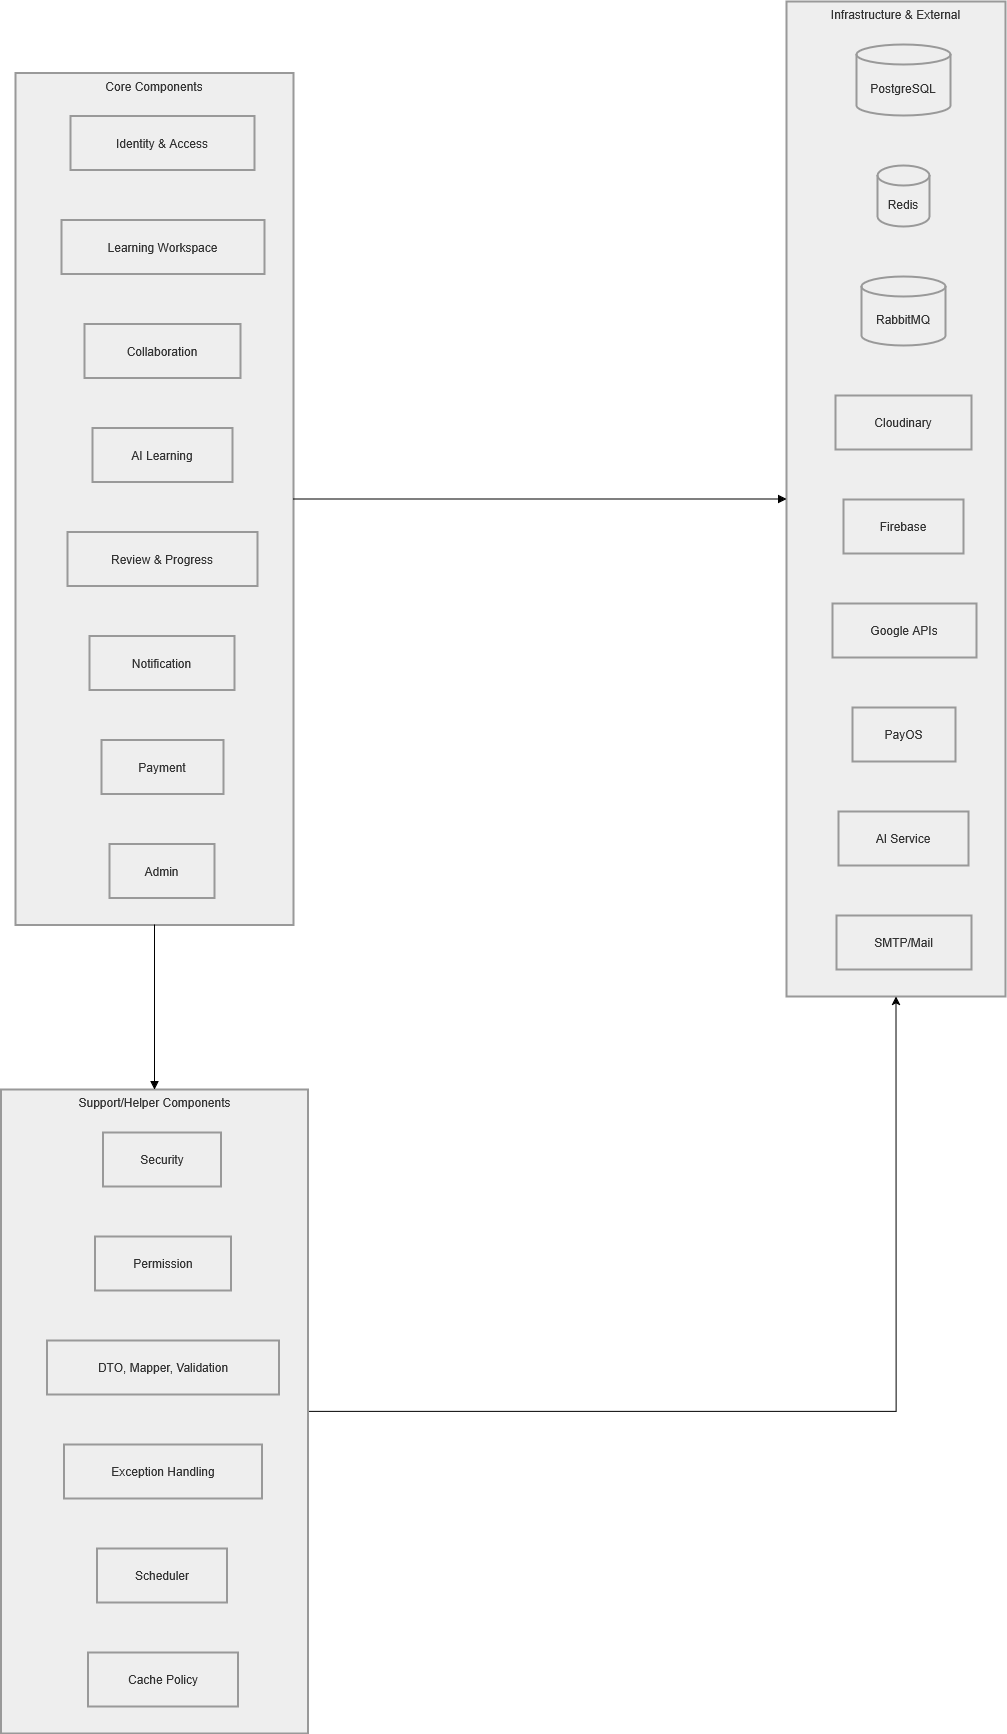
\includegraphics[width=0.95\textwidth,height=0.72\textheight,keepaspectratio]{images/chapter3/ProLearning_Arch-Detail_Components.drawio.png}
    \caption{Chi tiết các thành phần của hệ thống ProLearning Platform}
    \label{fig:prolearning-architecture-detail-components}
\end{figure}

\endgroup